%% LyX 1.3 created this file.  For more info, see http://www.lyx.org/.
%% Do not edit unless you really know what you are doing.
\documentclass[brazil,ruledheader]{abnt}
\usepackage[T1]{fontenc}
\usepackage[latin1]{inputenc}
\usepackage{abntcite}
\usepackage{graphicx}
\usepackage{multirow}
\usepackage{amssymb}
\newcommand{\reg}[1]{#1$^{\tiny{\circledR}}$}
\makeatletter
\usepackage{babel}
\makeatother
\begin{document}
\autor{Anderson Berg dos Santos Dantas}
\titulo{Sistema de Recomenda��o para clientes de v�deo locadoras baseado em redes Kohonen}
\orientador{Prof. Fernando Buarque de Lima Neto, PhD}

\comentario{Monografia apresentada como requisito parcial para obten��o do diploma de Bacharel em Engenharia da Computa��o pela Escola Polit�cnica de Pernambuco - Universidade de Pernambuco.}


\instituicao{Departamento de Sistemas e Computa��o \par Escola Polit�cnica de Pernambuco \par Universidade de Pernambuco}


\local{Recife - PE, Brasil}


\data{Novembro de 2009 }

% Folha de rosto sem o uso de \folhaderosto
\begin{titlepage}

\vfill
\begin{center}
\begin{figure}[!t]

\includegraphics[height=2.76cm]{polilogo-1}
\hfill

\includegraphics[height=1.58cm]{marca_dsc}
\end{figure}\ 
\vfill
\vspace{.10\textheight}
{\Huge Sistema de Recomenda��o para clientes \par de v�deo locadoras baseado em redes Kohonen}\\[3cm]

{\Large \par Trabalho de Conclus�o de Curso \par Engenharia da Computa��o}\\[4cm]
\begin{flushleft}
{\large Anderson Berg dos Santos Dantas}\\
{\large Orientador: Prof. Fernando Buarque de Lima Neto, PhD}
\end{flushleft}

\vfill
\begin{figure}[!b]
\begin{center}

\includegraphics[height=2.76cm]{brasao_upe}
\end{center}
\end{figure}\ 
\end{center}

\end{titlepage}

\folhaderosto

%\begin{folhadeaprovacao}
%Monografia de Projeto Final de Gradua��o sob o t�tulo \textit{``\ABNTtitulodata''},
%defendida por \ABNTautordata~e aprovada em \ABNTdatadata, em Vit�ria,
%Estado do Esp�rito Santo, pela banca examinadora constitu�da pelos
%professores: \setlength{\ABNTsignthickness}{0.4pt}

%\assinatura{Prof. Msc. S�rgio A. A. de Freitas\\ Orientador} \assinatura{Prof. Dr. %Fl�vio Miguel Varej�o\\ Universidade Federal do Esp�rito Santo} \assinatura{Prof. Dr. %Raul Henriques Cardoso Lopes\\ Universidade Federal do Esp�rito Santo}
%\end{folhadeaprovacao}
\begin{resumo}

\end{resumo}
\begin{abstract}

\end{abstract}

\chapter*{Dedicat�ria}

A Deus e minha fam�lia, pois me ensinaram os passos que devo seguir.

\chapter*{Agradecimentos}

Agrade�o a Deus pelo amor e ajuda a todo momento durante a gradua��o.

Aos meus pais que sempre me apoiaram e me encorajaram a cursar uma faculdade. Agradecimento especial � minha m�e, que tem sido uma forte coluna.

Ao meu irm�o pela compreens�o e ajuda. � minha irm�.

Agrade�o aos colegas e professores pela confian�a e credibilidade que me ajudaram a prosseguir.

Ao meu orientador que acreditou a todo momento que era poss�vel realizar este trabalho.


\tableofcontents{}
\listoffigures



\listoftables

\chapter{Introdu��o}\label{cap:introducao}
\section{Caracteriza��o do Problema}
A tecnologia, principalmente a internet, tem mudado a forma de fazer neg�cios na ind�stria do entretenimento. V�-se atualmente, a migra��o do mercado f�sico para o virtual. Muitas lojas disponibilizam os seus produtos � venda atrav�s de s�tios na grande rede de computadores, outras, ainda, possuem apenas as lojas virtuais. Uma das vantagens dessas lojas � o fato de, por n�o precisar de um ambiente f�sico para vendas, o n�mero de produtos oferecidos � muito maior \cite{Anderson2006}, que leva a um problema conhecido com sobrecarga de informa��o. 

Diante de tanta diversidade, o cliente, que vai adquirir um produto em s�tios de com�rcio eletr�nico, frequentemente precisa de aux�lio para encontrar o que deseja. Al�m das ferramentas de busca, as grandes lojas virtuais disponibilizam uma forma de mostrar ao cliente informa��es personalizadas sobre produtos que podem interess�-lo, que � o sistema de recomenda��o. Os sistemas de recomenda��o podem sugerir produtos utilizando diversos aspectos, como compras anteriores de determinado cliente ou opini�es de outros clientes sobre os produtos da loja. Desta feita, os sistemas de recomenda��o criam lojas personalizadas para o perfil de cada cliente. A personaliza��o incorpora algo muito importante para o neg�cio que � a fideliza��o do cliente.

Em v�deo locadoras � comum a dificuldade de sugerir novos filmes para clientes, mesmo para os clientes mais antigos. � dif�cil o funcion�rio de um estabelecimento identificar o perfil do cliente a partir de filmes j� locados e quais foram suas prefer�ncias. O cliente, por muitas vezes, segue a opini�o de outras pessoas para saber se um determinado t�tulo � um bom filme ou n�o, opini�o que, geralmente, n�o corresponde ao perfil do cliente. Atualmente as locadoras de dvd est�o disponibilizando loca��es atrav�s de p�ginas na internet com a vantagem da entrega a domic�lio. Fato que dificulta ainda mais a obten��o de opini�es de terceiros pelo cliente. Sistemas de recomenda��o podem trazer todas as suas vantagens para v�deo locadoras tanto f�sicas como virtuais, auxiliando o cliente a fazer a melhor escolha. Isso leva a uma personaliza��o da v�deo locadora na vis�o do cliente.
	
\section{Motiva��es}
O que motivou o presente trabalho foi a possibilidade de tornar a escolha de um filme para loca��o uma experi�ncia mais simples e interessante. O cliente poder� direcionar suas escolhas a partir das informa��es que o sistema ir� fornecer, todas baseadas no hist�rico de t�tulos locados na loja. Este trabalho tenta minimizar o problema da sobrecarga de informa��o provendo o cliente de par�metros que possam identificar o seu perfil.
\section{Objetivos e Metas}
O objetivo deste trabalho � desenvolver um sistema de recomenda��o simples para clientes que frequentam v�deo locadoras. O sistema visa facilitar e agilizar a escolha de um filme pelo cliente, diminuindo as chances de desperd�cio de dinheiro em algo que n�o lhe agrada. Al�m de oferecer um servi�o diferenciado ao cliente, a v�deo locadora ir� se beneficiar pela fideliza��o do mesmo, j� que ocorre uma personaliza��o do servi�o. Temos como meta construir um mapa auto-organiz�vel de Kohonen distribuindo o hist�rico de loca��es de um determinado cliente de maneira que este possa visualizar todo seu hist�rico de forma gr�fica. Quando o cliente desejar realizar uma loca��o o mapa ir� mostrar o lugar que este novo filme se insere e seus principais vizinhos que caracterizam os filmes mais relacionados ao que ele deseja locar.
\section{Organiza��o do Documento}
\subsection{Cap�tulo 2: Revis�o Bibliogr�fica}
Ser�o apresentados os principais conceitos em que se baseia o modelo proposto por este trabalho. O cap�tulo inicia com uma revis�o sobre Sistemas de Recomenda��o, abordando as principais t�cnicas de recomenda��o, suas vantagens e desvantagens e modelos propostos para solu��o de problemas na recomenda��o. A segunda parte do cap�tulo apresenta um tipo especial de redes neurais artificiais: as redes auto-organiz�veis ou redes SOM (\textit{self-organizing map}). Ser� abordado o modelo de redes SOM introduzido por Kohonen.
\subsection{Cap�tulo 3: Modelo Proposto}
Descreve a proposta central do modelo, al�m do algoritmo que foi desenvolvido.
\subsection{Cap�tulo 4: Configura��es dos Experimentos e An�lise dos Resultados}
Neste cap�tulo ser�o expostos os experimentos realizados com o modelo e os resultados obtidos para comprovar a funcionalidade do trabalho.
\subsection{Cap�tulo 5: Conclus�o e Trabalhos Futuros}
Considera��es finais, dificuldades enfrentadas durante o desenvolvimento e propostas de continuidade do trabalho.
\chapter{Fundamenta��o Te�rica}\label{cap:fundamentacao}
Neste cap�tulo iremos apresentar os principais conceitos que ajudar�o na compreens�o do resto do documento. Primeiramente ser�o abordadas as caracter�sticas de sistemas de recomenda��o estabelecidos na literatura. Tamb�m ser�o abordadas as principais t�cnicas de recomenda��o, apontando suas vantagens, principais problemas e solu��es propostas por diversos autores a fim de solucionar essas falhas. Posteriormente ser�o apresentados os mapas auto-organiz�veis, em especial os mapas de Kohonen, definindo sua arquitetura e o algoritmo de aprendizado.

\section{Sistemas de Recomenda��o}
O uso de sistemas informatizados, principalmente da internet, resulta em um grande volume de informa��o sendo criada e transmitida no mundo todo \cite{Terveen2001}. Um estudo realizado em 2003 por pesquisadores da Universidade da Calif�rnia \cite{Lyman2003} estimou que cinco exabytes de informa��o foram criados no ano de 2002, onde a maior parte � armazenada em dispositivos magn�ticos, em especial discos r�gidos. Nasceu, ent�o, a necessidade da cria��o de mecanismos que tenham a capacidade de filtrar ou recuperar rapidamente informa��o. Com o objetivo de facilitar a busca por informa��o foram criados mecanismos que pudesse indexar documentos na internet e, rapidamente, recuper�-los, trazendo ao usu�rio aquilo que ele precisa. Tais mecanimos s�o as ferramentas de busca como o google (www.google.com), que seleciona documentos na internet a partir de crit�rios que o usu�rio expressa atrav�s de palavras-chave.

O com�rcio, principalmente a ind�stria do entretenimento, tem se beneficiado com a evolu��o da tecnologia. As lojas n�o precisam mais ter espa�o f�sico, � poss�vel realizar vendas e fazer negocia��es com seguran�a atrav�s da internet. A \textit{Itunes Store} possui mais de 10 milh�es de m�sicas dispon�veis para venda atrav�s de \textit{download}. As grandes lojas de departamentos possuem lojas virtuais para com�rcio eletr�nico, algumas delas nem possuem lojas f�sicas, apenas os s�tios na internet onde podem vender seus produtos. Casos de sucesso no Brasil s�o as Americanas.com (www.americanas.com.br) e o Submarino (www.submarino.com.br). Sem a necessidade de ter espa�o f�sico ou prateleiras, os itens que podem ser colocados � venda s�o de um n�mero superior se comparado a uma loja convencional \cite{Anderson2006}. Diante de tantas possibilidades, como ir em busca da melhor informa��o? Qual produto vale a pena adquirir? Qual filme ou m�sica escolher? Frequentemente as pessoas procuram opini�es de terceiros, como amigos e familiares que j� tiveram uma experi�ncia com determinado produto ou servi�o. Podem, ainda, procurar por resenhas em jornais e revistas, ou pedir a opini�o do dono de uma livraria ou v�deo locadora. Por�m, nenhum deles pode fazer recomenda��es de acordo com prefer�ncias pessoais.

Filtrar toda a informa��o recebida por um usu�rio, raramente � uma tarefa simples e eficiente. Um dos primeiros sistemas de filtragem criados foi o Tapestry \cite{Goldberg1992}. Este sistema filtrava documentos enviados para a caixa de \textit{emails} de um usu�rio. O Tapestry analisava, n�o somente o conte�do dos textos, mas tamb�m o interesse que outros usu�rios tinham por esses documentos. Os idealizadores desse projeto cunharam o termo ''filtragem colaborativa'', propondo um sistema onde a filtragem de documentos seria realizada com aux�lio de grupos de pessoas com o mesmo interesse. Atualmente, os s�tios de com�rcio eletr�nico disponibilizam para seus clientes ferramentas computacionais com o objetivo de auxili�-los no momento da compra. Essas ferramentas caracterizam os sistemas de recomenda��o. Tais sistemas consistem em mostrar ao usu�rio produtos que sejam de seu interesse, alguns sistemas ainda fornecem opini�es de outros clientes sobre aqueles produtos. 

Auxiliar o cliente mostrando produtos relacionados a suas prefer�ncias � uma forma de personaliza��o. A personaliza��o � uma caracter�stica do \textit{marketing} direto. Diferente do \textit{marketing} de massa, cujo objetivo � alcan�ar o maior n�mero de pessoas atrav�s dos diversos tipos de m�dia, o \textit{marketing} direto � mais pessoal, ele se interessa pelo indiv�duo. Personalizar resulta na fideliza��o do cliente, que � um grande diferencial entre empresas concorrentes \cite{Filho2006}. \cite{Reategui2005} cita algumas estrat�gias utilizadas pelos s�tios de com�rcio eletr�nico para recomenda��o de produtos:

\begin{itemize}
	\item Listas de recomenda��o: A loja mant�m listas de produtos, como itens mais vendidos, itens que t�m a melhor avalia��o entre os clientes ou lista de presentes, entre outros.
	\item Avalia��o de usu�rios: Consiste em se obter notas do produto por clientes que j� o adquiriram, al�m dessa avalia��o usu�rios podem deixar coment�rios sobre determinado produto (Figura \ref{avaliacao}).
	\item Suas recomenda��es: O s�tio oferece alguns produtos baseado em interesses do cliente. Aqui pode-se ter dois tipos de recomenda��o: impl�cita, onde o s�tio oferece produtos de acordo com o hist�rico de compras do cliente, ou expl�cita, onde o usu�rio determina quais s�o suas prefer�ncias (Figura \ref{amazon_tbcompra}).
	\item ''Clientes que adquiriram um produto X, tamb�m compraram Y'': O sistema de recomenda��o cria associa��es entre produtos avaliados por usu�rio para oferecer produtos relacionados ao que o cliente est� adquirindo no momento (Figura \ref{also_bought}).
	\item Associa��o por conte�do: Este tipo de recomenda��o � feita baseado no conte�do de determinado item. Por exemplo: Clientes que compraram um livro de Redes de Computadores tamb�m compraram um livro sobre a linguagem Java.
\end{itemize}

\begin{figure}[htbp]
	\centering
		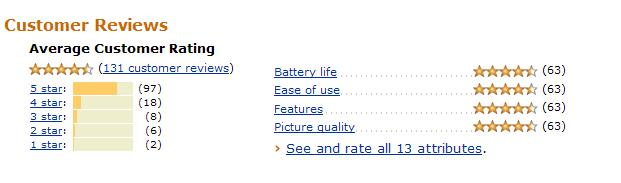
\includegraphics[width=1.00\textwidth]{imagens/avaliacao.JPG}
	\caption{Avalia��es de usu�rios no site da Amazon para uma c�mera fotogr�fica.}
	\label{avaliacao}
\end{figure}

\begin{figure}[htbp]
	\centering
		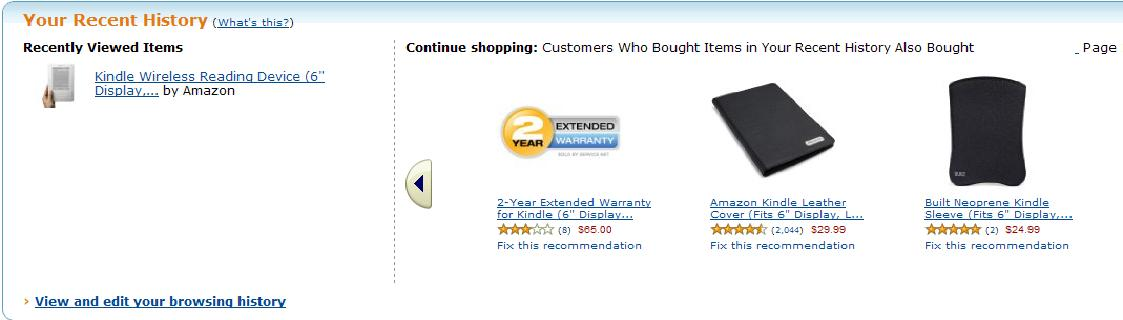
\includegraphics[width=1.10\textwidth]{imagens/amazon_tbcompra.JPG}
	\caption{Recomenda��es da Amazon de acordo com o hist�rico do cliente.}
	\label{amazon_tbcompra}
\end{figure}

\begin{figure}[htbp]
	\centering
		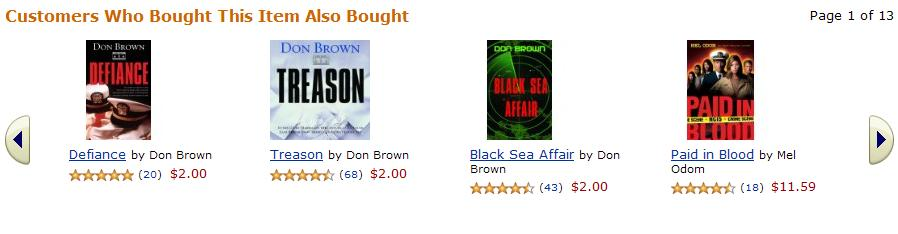
\includegraphics[width=1.00\textwidth]{imagens/also_bought.JPG}
	\caption{Associa��o de produtos por clientes no site da Amazon}
	\label{also_bought}
\end{figure}


\subsection{T�cnicas de recomenda��o}
Diversas t�cnicas foram definidas na literatura com o objetivo de identificar padr�es de comportamento e filtragem de informa��o para obter recomenda��es e personaliza��o para o usu�rio. As tr�s t�cnicas mais utilizadas em sistemas de recomenda��o s�o a filtragem baseada em conte�do, a filtragem colaborativa e a filtragem h�brida, que procura conciliar as vantagens das duas anteriores atacando seus principais problemas.

\subsubsection{Filtragem baseada em conte�do}
A filtragem baseada em conte�do tem suas ra�zes no processo chamado de recupera��o de informa��o, onde o usu�rio apresenta ao sistema um formul�rio e recebe, como resultado, documentos associados a esses crit�rios \cite{Balabanovic1997}. O principal objetivo da recupera��o de informa��o � encontrar documentos que casem com um determinado crit�rio de busca \cite{Gabrielsson2006}. Em um sistema de recupera��o de informa��o, o usu�rio fornece ao sistema palavras-chave que representam seus interesses ou necessidades atuais na busca por informa��o. O sistema ent�o, realiza um busca por essas palavras em documentos armazenados numa base e retorna os documentos mais relevantes para aquela busca. 

Ao contr�rio da recupera��o de informa��o, a filtragem de informa��o mant�m um perfil do usu�rio filtrando todo novo item relacionado a seus interesses a longo prazo, enquanto a recupera��o de informa��o representa interesses de curto prazo \cite{Herlocker2000}. Os atuais sistemas de recomenda��o t�m sua origem nos sistemas de filtragem de informa��o. Em 1982, \cite{Denning1982} j� apontava para o problema da filtragem de informa��o. Neste artigo, Denning alerta para a facilidade de produ��o e transmiss�o de informa��o e que � necess�rio uma aten��o maior para o processo de controlar e filtrar informa��o. Filtragem de informa��o e filtragem baseada em conte�do s�o termos semelhantes e ambos possuem o mesmo objetivo: filtrar itens de acordo com seu conte�do \cite{Gabrielsson2006}. 

Na filtragem baseada em conte�do as recomenda��es s�o feitas apenas baseadas em um perfil do usu�rio previamente constru�do a partir da an�lise do conte�do de itens que este qualificou ou mostrou algum interesse no passado \cite{Balabanovic1997}. Quando um usu�rio de um s�tio de com�rcio eletr�nico, por exemplo, entra na p�gina da loja e exp�e suas necessidades atrav�s de palavras-chave na ferramenta de busca, ele est� realizando uma recupera��o de informa��o, pois o sistema vai procurar produtos que satisfa�am os simplesmente os crit�rios apresentados no momento. Quando este mesmo s�tio armazena o perfil do usu�rio e apresenta produtos semelhantes aos que este usu�rio mostrou interesse no passado, caracteriza uma filtragem de informa��o. Uma das t�cnicas mais populares para representa��o dos itens em sistemas de filtragem baseada em conte�do � a TF-IDF (Term-frequency Inverse-Document-Frequency). Esta t�cnica realiza compara��o e c�lculo de similaridade a partir da frequ�ncia de ocorr�ncia de palavras-chave nos textos \cite{Filho2006}. Para cria��o do perfil do usu�rio, normalmente s�o utilizadas t�cnicas de computa��o inteligente, que podem aprender o comportamento de determinado usu�rio, por exemplo, algoritmos de classifica��o podem indentificar e fazer a divis�o entre itens que o usu�rio gosta e itens que ele n�o gosta \cite{Gabrielsson2006}. O \textit{feedback} � muito importante na fase de aprendizado, podendo ser expl�cito, quando o usu�rio qualifica o item que lhe foi oferecido, ou impl�cito, quando o usu�rio demonstra interesse no item finalizando com a compra \cite{Terveen2001}. Exemplos de sistemas que utilizam a filtragem baseada em conte�do s�o o NewsWeeder \cite{Lang1995} e o InfoFinder \cite{Krulwich1996}.

A filtragem baseada em conte�do possui pontos positivos e negativos, dentre suas vantagens pode-se citar: (i) n�o � necess�rio que um novo item tenha algum tipo de qualifica��o, bastando apenas que este seja semelhante ao perfil do usu�rio e (ii) por avaliar a semelhan�a entre todos os itens, a filtragem baseada em conte�do n�o se restringe a itens j� avaliados por outros usu�rios. Os principais problemas apresentados pela filtragem baseada em conte�do s�o: (i) as representa��es de conte�do de um item n�o conseguem capturar alguns aspectos, como qualidade de um texto, no caso sistemas de recomenda��o de documentos, ou informa��es de multim�dia, no caso de sistemas que recomendam p�ginas da internet \cite{Balabanovic1997}; (ii) o segundo ponto negativo da filtragem baseada em conte�do � a superespecializa��o. Como esse tipo de filtragem leva em considera��o itens que o usu�rio j� mostrou interesse, as recomenda��es ficam restritas a itens similares a itens j� qualificados pelo usu�rio.

\subsubsection{Filtragem colaborativa}
A filtragem colaborativa � a t�cnica de recomenda��o mais comum e a mais largamente utilizada \cite{Burke2002}. A abordagem da filtragem colaborativa � recomendar itens baseados na similaridade entre usu�rios, deferentemente da filtragem baseada em conte�do, que realiza similaridade entre itens. Basicamente, � formado um conjunto de usu�rios denominados ''vizinhos mais pr�ximos'', que possuem itens classificados de forma semelhante ao usu�rio atual. Os itens que ser�o recomendados s�o itens que foram bem qualificados por esse grupo de usu�rios, partindo do pressuposto que esse grupo de usu�rios t�m prefer�ncias em comum com o usu�rio atual. A priori, neste tipo de t�cnica nenhuma informa��o sobre os itens em si � conhecida, as recomenda��es s�o baseadas na semelhan�a entre os usu�rios \cite{Balabanovic1997}. Segundo descreve \cite{Burke2002}: ''O perfil de um usu�rio num sistema colaborativo consiste em um vetor de itens e suas qualifica��es, que � aperfei�oado na medida que o usu�rio interage com o sistema ao longo do tempo.'' 

Um dos primeiros sistemas a utilizar a filtragem colaborativa foi o Tapestry \cite{Goldberg1992}, j� mencionado anteriormente neste trabalho. A id�ia do Tapestry � fazer com que as pessoas colaborem entre si para realizar filtragens descrevendo suas percep��es a documentos que leram. Essas percep��es s�o armazenadas em coment�rios ou anota��es que podem ser consultadas por qualquer outro usu�rio. Uma forma de utiliza��o desse sistema seria um usu�rio buscar documentos que outro determinado usu�rio aprovou. Os principais representantes de sistemas que utilizam filtragem colaborativa, al�m do Tapesty, s�o o GroupLens \cite{Resnick1994}, Ringo \cite{Shardanand1995} e Bellcore \cite{Hill1995}. Podem-se citar algumas vantagens deste tipo de t�cnica:

\begin{itemize}
	\item Como as recomenda��es s�o baseadas em avalia��es de outros usu�rios � poss�vel tratar diferentes tipos de conte�do, n�o somente documentos textuais.
	\item A qualidade das recomenda��es � superior se comparado a sistemas que utilizam filtragem baseada em conte�do. A justificativa est� no fato de sistemas automatizados n�o serem eficientes em analisar a qualidade de um produto, por exemplo, mas quando se baseia na avalia��o de outros usu�rios � poss�vel produzir recomenda��es de qualidade.
\end{itemize}

Algumas das desvantagens da filtragem colaborativa s�o:

\begin{itemize}
	\item Se um novo item � introduzido no sistema, n�o ser� recomendado at� que um dos usu�rios o avalie. O que traz outra consequ�ncia: se o n�mero de usu�rios do sistema � reduzido em rela��o � quantidade de itens, ocorre um problema de cobertura, ou seja, a cole��o de itens que podem ser recomendados ser� resumida.
	\item Outro problema em sistemas utilizando filtragem colaborativa ocorre quando h� um usu�rio cujas prefer�ncias diferem dos demais usu�rios, ou seja, n�o h� vizinhos semelhantes ao usu�rio ativo, ocasionando em recomenda��es pobres.
\end{itemize}

\subsubsection{Filtragem h�brida}
A abordagem da filtragem h�brida consiste em associar duas ou mais t�cnicas de recomenda��o com o objetivo de tratar os principais problemas inerentes a cada uma delas. \cite{Burke2002} realizou um estudo sobre sistemas de recomenda��o h�bridos. Neste artigo ele aponta sete combina��es poss�veis entre t�cnicas de recomenda��o:

\begin{enumerate}
	\item Ponderado: A avalia��o de um item � a combina��o do resultado de todas as t�cnicas presentes no sistema. O sistema P-Tango \cite{Claypool1999} � um exemplo de uso desta t�cnica. A proposta do P-Tango � combinar as recomenda��es da filtragem baseada em conte�do e da filtragem colaborativa atrav�s de m�dias ponderadas. Os pesos s�o ajustados de acordo com o peso de cada recomenda��o, isto �, ao passo que o n�mero de usu�rios e avalia��es de um determinado item cresce, a filtragem colaborativa tem seu peso aumentado.
	\item Alternado: O sistema se utiliza de um crit�rio para alternar entre as t�cnicas de recomenda��o. Por exemplo, se uma filtragem baseada em conte�do n�o retorna resultados satisfat�rios, ent�o a recomenda��o � feita com a filtragem colaborativa.
	\item Misto: Neste tipo de combina��o, o sistema apresenta recomenda��es de diferentes t�cnicas numa mesma listagem. O sistema PTV \cite{Smyth2001} utiliza a filtragem baseada em conte�do baseado nas descri��es de programas de TV e a filtragem colaborativa baseado na prefer�ncia de outros usu�rios, o resultado das recomenda��es � uma combina��o dos resultados das duas filtragens.
	\item Combina��o de caracter�sticas: Trata informa��es de um tipo de recomenda��o como simples caracter�sticas que s�o utilizadas por outra t�cnica para retornar recomenda��es mais significativas. \cite{Basu1998} apresenta um sistema de recomenda��o de filmes onde as informa��es da filtragem colaborativa (denominadas, neste artigo, caracter�sticas colaborativas) s�o influenciadas pelo conte�do agregado aos filmes. Desta forma, � poss�vel agrupar usu�rios semelhantes e que gostem do mesmo g�nero de filmes.
	\item Cascata: Nesta combina��o, uma t�cnica, primeiramente, produz suas recomenda��es e uma segunda t�cnica � usada para refinar os resultados da anterior.
	\item Acr�scimo de caracter�stica: Primeiramente uma t�cnica � aplicada para gerar classifica��es para um item, ent�o estas informa��es s�o incorporadas na t�cnica seguinte.
	\item \textit{Meta-level}: Esta abordagem utiliza o modelo criado por uma t�cnica como entrada para outra t�cnica. No acr�scimo de caracter�stica, um modelo gera caracter�sticas para serem usadas como entrada para outro modelo, na abordagem \textit{meta-level} o modelo completo � utilizado como entrada para outro modelo.
\end{enumerate}

\section{Mapas auto-organiz�veis}
O principal objetivo das redes neurais artificiais (RNAs) � aprender com o ambiente em que est�o inseridas para adquirirem a capacidade de adapta��o �s mudan�as nesse ambiente. O tipo de aprendizado das redes neurais pode ser dividido em duas classes: aprendizado supervisionado e aprendizado n�o-supervisionado. O m�todo mais comumente utilizado � o aprendizado supervisionado, onde, al�m da entrada, a sa�da desejada para a rede s�o fornecidas por um supervisor externo \cite{Braga2000}. O objetivo � fazer o ajuste de par�metros de forma que a rede possa representar novas entradas corretamente. O m�todo de aprendizado supervisionado se limita, por�m, a aplica��es onde tanto os dados de entrada como as respostas desejadas s�o conhecidos. Algumas aplica��es necessitam que o treinamento seja realizado sem um supervisor para a rede, todo o conhecimento deve ser adquirido somente atrav�s das entradas. Diversos algoritmos foram desenvolvidos para treinar redes sem supervis�o, este trabalho ir� tratar de um deles: os modelos \textit{self-organizing} ou auto-organiz�veis.

Os mapas \textit{self-organizing}, SOM (\textit{Self-organizing maps}) foram propostas por Teuvo Kohonen \cite{Kohonen1989}. A estrutura b�sica dessas redes � formada por uma camada de entrada, constitu�da de padr�es fonte, e uma camada de sa�da que representa as entradas. N�o h� camadas escondidas (hidden layer) no modelo de mapas auto-organiz�veis como em outros tipos de redes neurais. A inspira��o para o desenvolvimento das redes SOM est� no mapa topologicamente organizado do c�rtex cerebral de animais mais desenvolvidos. O c�rtex cerebral humano � organizado de acordo com fun��es espec�ficas, como fala e vis�o (Figura \ref{cortex}). Desta forma, neur�nios que lidam com o mesmo tipo de est�mulo est�o localizados pr�ximos uns dos outros. O modelo de Kohonen consiste em um mapa, onde os n�s ou nodos que est�o topologicamente pr�ximos respondem a est�mulos semelhantes, ou seja, padr�es de entrada que possuem similaridade entre si. 

\begin{figure}[htbp]
\begin{center}
		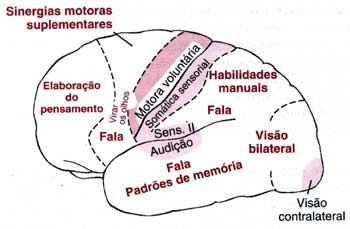
\includegraphics[width=0.50\textwidth]{imagens/cortex.jpg}
	\caption{C�rtex cerebral humano}
	\label{cortex}
\end{center}
\end{figure}

Na arquitetura de uma rede SOM, os nodos s�o dispostos em uma grade ou reticulado, geralmente bidimensional ou unidimensional, com raras exce��es, h� redes tridimensionais ou n-dimensionais. No modelo bidimensional, os neur�nios est�o organizados em linhas e colunas, como mostra a Figura \ref{mapa_som}. Cada nodo possui um conjunto de pesos que representam as sinapses do neur�nio biol�gico, esses pesos s�o ajustados de maneira que o nodo represente um dado padr�o de entrada. Os nodos de uma rede SOM funcionam como um extrator de caracter�sticas, quanto mais o vetor de pesos de um neur�nio for semelhante a um padr�o de entrada, maior ser� sua sa�da e mais representativo este nodo ser� para a entrada \cite{Braga2000}. 

\begin{figure}[htbp]
	\centering
		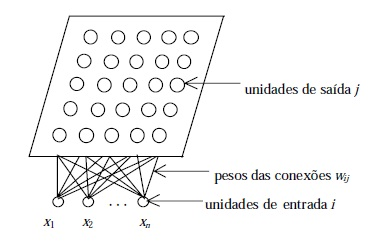
\includegraphics[width=0.60\textwidth]{imagens/mapa_som.jpg}
	\caption{Rede SOM bidimensional}
	\label{mapa_som}
\end{figure}

As redes SOM utilizam um processo de aprendizado competitivo, no qual os neur�nios da camada de sa�da competem entre si para representar um dado padr�o de entrada, assim, apenas um neur�nio de sa�da ou neur�nio por grupo estar� ativo a qualquer instante de tempo. O neur�nio que se sobressai entre os outros para representar a entrada � chamado de vencedor e a competi��o � chamada de \textit{winner-takes-all}, o vencedor leva tudo. Para implementar esta competi��o s�o normalmente utilizadas conex�es laterais inibit�rias entre os neur�nios de sa�da. O modelo para esse tipo de conex�o tamb�m prov�m das c�lulas do c�rtex cerebral, onde a ordena��o topol�gica dos neur�nios se d� gra�as ao \textit{feedback} lateral entre as c�lulas. Em RNAs este \textit{feedback} � modelado por uma fun��o chamada chap�u mexicano. Segundo esta fun��o, as intera��es laterais entre os neur�nios podem ser divididas em tr�s regi�es distintas, como mostrado na Figura \ref{mexican_hat}: (1) �rea excitat�ria, vizinhos que est�o mais pr�ximos ao neur�nio atual; (2) �rea inibit�ria, vizinhos que est�o fora da �rea anterior, mas inclu�dos numa segunda �rea; e (3) �rea levemente excitat�ria, que rodeia a �rea inibit�ria, esta terceira �rea geralmente � ignorada.

\begin{figure}[htbp]
	\centering
		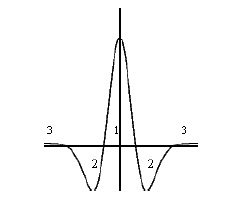
\includegraphics[width=0.40\textwidth]{imagens/mexican_hat.jpg}
	\caption{Fun��o chap�u mexicano}
	\label{mexican_hat}
\end{figure}
 
Para simular o efeito da fun��o chap�u mexicano, a rede SOM utiliza o conceito de vizinhan�a topol�gica dos neur�nios vencedores. Quando um neur�nio vence a competi��o e � o escolhido para representar o padr�o de entrada, ele tem seus pesos ajustados de forma a se aproximar mais da entrada, com o conceito de vizinhos topol�gicos, al�m do neur�nio vencedor ter seus pesos ajustados, os neur�nios localizados na vizinhan�a tamb�m t�m seus pesos ajustados.

Como dito anteriormente, o treinamento de redes SOM � competitivo e n�o-supervisionado. Primeiramente os pesos dos neur�nios do mapa s�o inicializados com valores aleat�rios, que ser�o ajustados ao longo do algoritmo de aprendizado, de forma que se aproximem dos padr�es de entrada. Em seguida � apresentado um padr�o \emph{p} � rede, neste momento a rede define o neur�nio que melhor representa esta entrada, caracterizando o neur�nio vencedor. Para a escolha do neur�nio vencedor � definida uma fun��o de ativa��o que � baseada na dist�ncia entre o peso do neur�nio e o vetor de entrada. A fun��o de ativa��o mais conveniente para a rede SOM � baseada na dist�ncia euclidiana \cite{Kohonen1990}, apresentada na equa��o \ref{dist_euclid}:

\begin{equation}
y_{j} = \sum\limits_{i=1}^n \left\|x_{i} - w_{ji} \right\|
\label{dist_euclid}
\end{equation}
onde $y_{j}$ representa a sa�da do neur�nio $j$, $x$ � o vetor de entrada e $w_{ji}$ � o peso do neur�nio  $j$ associado ao elemento de entrada $x_{i}$.

O neur�nio que possui a menor dist�ncia � escolhido como o vencedor e ir� representar o padr�o de entrada. Ap�s essa escolha d�-se in�cio ao processo de atualiza��o dos pesos. Nesta fase o neur�nio vencedor e os vizinhos definidos pelo raio ou �rea de vizinhan�a atualizam seus pesos. A fim de implementar a intera��o lateral, � definida uma regi�o de vizinhan�a $N_{c}$, tendo como centro o neur�nio $c$, estabeleciso como vencedor pela fun��o de ativa��o. Todos os neur�nios internos a essa vizinhan�a ter�o os pesos atualizados, enquanto neur�nios fora do limite ser�o deixados intactos. O valor do raio ou tamanho de $N_{c}$ deve, inicialmente, ser alto e diminuir monotonicamente no tempo \cite{Kohonen1990}. Tal valor pode, ao final do processo, abranger apenas o neur�nio central ($N_{c} = \{c\}$), como se pode observar na Figura \ref{vizinho}. A equa��o \ref{atualiza_pesos} mostra como s�o atualizados os pesos do neur�nio vencedor e dos neur�nios vizinhos.

\begin{equation}
w_{ji}(t+1) = 
\left\{ \begin{array}{l}
w_{ji}(t) + \alpha(t) (x_{i}(t) - w_{ji}(t)), \mbox{ se } j \in N_{c}(t) \\
w_{ji}(t), \mbox{ se } j \notin N_{c}(t)
\end{array} \right.
\label{atualiza_pesos}
\end{equation}
onde $\alpha(t)$ � o valor da taxa de aprendizado $0<\alpha(t)<1$, que decresce no tempo.

Como alternativa pode ser introduzida uma fun��o de vizinhan�a do neur�nio vencedor, definido pela seguinte equa��o, com $r_{c}$ e $r_{j}$ como as coordenadas dos neur�nios $c$ (neur�nio central ou vencedor) e $j$, respectivamente:

\begin{equation}
h_{ci}(t) = h_{0} \exp(-\left\|r_{i} - r_{c} \right\|^2 / \sigma^2)
\end{equation}
onde $h_{0} = h_{0}(t)$ e $\sigma = \sigma(t)$ s�o fun��es que devem decrescer no tempo. O par�metro $\sigma(t)$ corresponde ao raio de $N_{c}(t)$. O ajuste de pesos passa ent�o a ser calculado desta forma:

\begin{equation}
w_{ji}(t+1) = w_{ji}(t) + h_{ci} (x_{i}(t) - w_{ji}(t))
\label{ajuste}
\end{equation}

\begin{figure}[htbp]
	\centering
		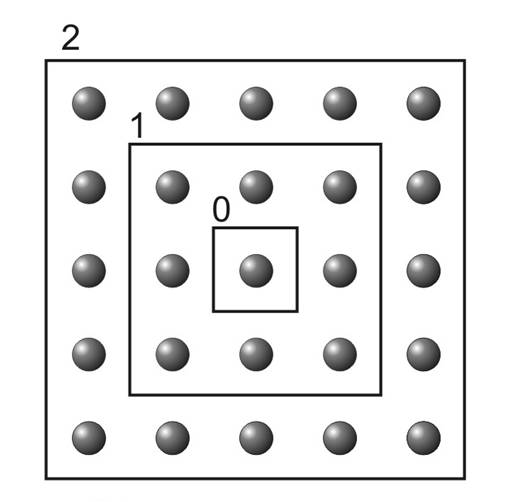
\includegraphics[width=0.30\textwidth]{imagens/vizinho.jpg}
	\caption{Exemplo de vizinhan�a, onde o instante 2 � menor que o instante 1, que por sua vez � menor que o instante 0}
	\label{vizinho}
\end{figure}

Segundo estudos e experi�ncias na escolha dos par�metros, Kohonen \cite{Kohonen1990} recomenda que o valor inicial de $\alpha(t)$ (taxa de aprendizado da rede) deve estar pr�ximo de 1 e decair monotonicamente durante os primeiros 1000 ciclos da fase de aprendizado, por�m mantendo o valor acima de 0,1. A regra para o decr�scimo de $\alpha(t)$ pode ser uma fun��o linear, exponencial ou inversamente proporcional a $t$, por exemplo: $\alpha(t) = 0.9(1-t/1000)$. � durante esta fase inicial do treinamento que ocorre a fase de ordena��o da rede. Nas fases seguintes ocorre o ajuste fino da rede, chamado de fase de converg�ncia. O n�mero de ciclos da fase de aprendizado deve ser razoavelmente grande. Uma regra emp�rica � que este n�mero deva ser 500 vezes maior que o n�mero de neur�nios na rede. O tamanho da vizinhan�a de um neur�nio n�o pode ser muito pequeno inicialmente, pois o mapa n�o teria uma boa ordena��o global. A princ�pio o raio ou tamanho inicial da vizinhan�a pode ser maior que a metade do tamanho do mapa.
\chapter{Modelo proposto}\label{cap:som}

Este trabalho visa apresentar um modelo para recomenda��o de filmes para cliente no ambiente de v�deo locadoras. O modelo proposto utiliza as redes SOM como descritas por Kohonen \cite{Kohonen1989} para auxiliar o usu�rio na escolha do filme.

Ap�s a descri��o dos conceitos e algoritmos apresentados no cap�tulo 2, ser� apresentado neste cap�tulo a contribui��o do modelo proposto.

O modelo de recomenda��o deste trabalho leva em considera��o a limita��o das v�deos locadoras no que tange aos conceitos gerais de sistemas de recomenda��o comuns. As informa��es que est�o dispon�veis num ambiente de locadora de filmes consideram somente o cliente como indiv�duo e n�o um grupo de clientes que podem contribuir juntamente para gerar recomenda��es. Portanto n�o h� o conceito de avalia��o de um item pelo usu�rio. Nos sistemas de locadoras comuns n�o existe um mecanismo onde o cliente possa dar sua nota para um filme de forma que outros clientes possam acompanhar essas avalia��es e ter um par�metro para a escolha de determinado t�tulo. Existe apenas a opini�o ''de boca'' de clientes que queiram expressar ou quando o funcion�rio da loja educadamente questiona sobre a satisfa��o do cliente. Mas nada � armazenado num banco de dados, nem � realizado um levantamento das opini�es de diversos clientes, com o prop�sito de identificar os melhores filmes.

A proposta deste trabalho � desenvolver um sistema que, baseado somente no hist�rico de loca��es de um cliente, possa conduz�-lo a uma escolha satisfat�ria no momento de locar um novo t�tulo. O sistema se baseia somente no conte�do dos filmes que j� foram locados por um determinado cliente, informa��es que podem ser facilmente obtidas. 

Como mencionado anteriormente, n�o existem avalia��es de clientes sobre os filmes nem par�metros que determinem as prefer�ncias desses clientes. Portanto, o modelo proposto n�o ambiciona gerar uma lista de recomenda��es diretas com t�tulos para o cliente, apenas auxili�-lo de forma a realizar uma escolha consciente baseado nas informa��es contidas nos filmes.

O modelo proposto consiste em uma rede SOM composta por filmes contidos no hist�rico de um cliente. Existe, portanto, um mapa SOM para cada cliente. A rede ir� distribuir os t�tulos em um mapa bidimensional, agrupando-os de acordo com semelhan�as entre informa��es fornecidas sobre os filmes.

Ap�s o treinamento da rede, os filmes locados por um cliente estar�o distribu�dos no mapa. O cliente deve, ent�o selecionar um filme do acervo da locadora e apresentar ao seu mapa individual. A rede ir� calcular a posi��o deste novo filme e ir� mostrar ao usu�rio 3 filmes que estejam pr�ximos �quele, determinando que h� semelhan�as entre esses quatro t�tulos. Esta � uma forma de auxiliar o cliente, pois ele pode avaliar se ir� gostar ou n�o do filme, partindo da satisfa��o que teve ao assistir os outros tr�s.

As informa��es que ser�o extra�das dos filmes s�o: g�nero, ano de lan�amento, n�mero de premia��es (Oscar, Globo de Ouro), quantidade de loca��es do filme.


\chapter{Experimentos e An�lise de Resultados}\label{resultados}
Este cap�tulo tem como objetivo descrever os experimentos realizados e resultados obtidos a partir da implementa��o do modelo descrito no Cap�tulo 3.

\section{Base de dados}
Como mencionado no cap�tulo anterior, o objetivo deste trabalho � auxiliar clientes na escolha de filmes em uma v�deo locadora. Foi desenvolvida uma rede auto-organiz�vel, segundo o modelo de Teuvo Kohonen \cite{Kohonen1990}, com o fim de aprender o comportamento do usu�rio e poder gui�-lo em sua escolha. Para a realiza��o dos testes foi utilizada uma base de dados real, extraindo as caracter�sticas que mais se adequam ao modelo proposto.

Inicialmente estava sendo negociada a obten��o dos dados de uma v�deo locadora da cidade, mas devido a entraves na pol�tica de seguran�a da empresa que fornece o sistema para esta locadora, n�o foi poss�vel coletar os dados reais para teste de campo do sistema. A alternativa encaminhada foi utilizar uma base, tamb�m real, dispon�vel abertamente na internet. A base de dados utilizada foi a MovieLens Data Set (http://www.grouplens.org), fornecida pelo grupo de pesquisa GroupLens Research. Essa base conta com 100.000 avalia��es para 1682 filmes por 943 usu�rios. A base MovieLens foi constru�da a partir do s�tio de recomenda��es de filmes: movielens.org. A base de dados MovieLens � assim organizada: 

\begin{itemize}
	\item Arquivo u.data: arquivo contendo 100.000 avalia��es de 943 usu�rios para 1682 filmes. Cada usu�rio avaliou, no m�nimo 20 t�tulos.
	\item Arquivo u.item: cont�m informa��es sobre os filmes, t�tulo, data de lan�amento e g�nero.
	\item Arquivo u.genre: lista de g�neros de filmes.
	\item Arquivo u.user: informa��o demogr�fica sobre os usu�rios: nome, idade, g�nero, profiss�o.
	\item Arquivos de treinamento e teste: a base u.data � dividida em dois tipos de arquivos com a rela��o de 80\%/20\% para treinamento e teste, respectivamente.
\end{itemize}

Para o escopo deste trabalho, n�o ser�o utilizadas as avalia��es dos usu�rios durante a fase de treinamento, pois fugiria ao objetivo que � fazer recomenda��es em ambientes de locadoras de filmes reais, onde n�o h� o conceito de avalia��o pelos clientes.

O ambiente de experimentos foi assim determinado:

Da base de filmes foram extra�dos o n�mero de identifica��o �nico do filme (ID), t�tulo do filme, ano de lan�amento, g�nero e n�mero de vezes que aparece no arquivo de avalia��es. Este �ltimo par�metro representa, para a realidade do presente trabalho, o n�mero de loca��es totais do filme na locadora. O arquivo de avalia��es dos usu�rios representa as loca��es de cada cliente, portanto o mapa � constru�do cruzando as informa��es destas duas tabelas.

O arquivo de testes representa os filmes que o cliente deseja locar, ent�o esses padr�es s�o apresentados ao sistema com a rede j� treinada. 

\section{Resultados}

Foram criadas tabelas para visualiza��o e estudo dos resultados obtidos com os experimentos realizados.

O primeiro t�tulo apresentado nas tabelas � o filme que o cliente deseja locar, os tr�s seguintes s�o os vizinhos mais pr�ximos no mapa, que indicam ser semelhantes ao primeiro. Para a avalia��o dos resultados foi considerada a nota ou avalia��o que o usu�rio deu ao filme. Por exemplo, na Tabela \ref{Cliente1_Shangai}, o cliente 1 deseja locar o filme \emph{Shangai Triad}. Quando apresentado este filme � rede, o cliente obteve como resposta os filmes: \emph{The White Balloon}, \emph{Belle de jour} e \emph{Jean de Florette}, evidenciando factualmente que estes filmes t�m similaridades com o primeiro. Observando os t�tulos que foram mostrados como relacionados, o cliente ir� avaliar se vale a pena alugar o filme \emph{Shanghai Triad}. Para avaliar esse resultado, observa-se a coluna \textbf{Avalia��o} da tabela, os filmes relacionados possuem avalia��o de 4, 3 e 5, respectivamente, indicando que o cliente teve satisfa��o razo�vel a �tima ao assist�-los. Portanto, a interpreta��o desse resultado � que o filme \emph{Shanghai Triad} provavelmente ir� agradar o cliente. A avalia��o para o filme \emph{Shanghai Triad} foi de 5, ou seja, a satisfa��o do usu�rio foi muito boa.

\begin{table}[htbp]
	\centering
	\caption{Resultados para o cliente 1 e o filme \emph{Shangai Triad}}
		\begin{tabular}{|l|c|c|c|c|}
		  \hline
			\textbf{T�tulo} & \textbf{G�nero} & \textbf{Ano} & \textbf{N�mero de loca��es} & \textbf{Avalia��o} \\
			\hline
			Shanghai Triad & Drama & 1995 & 20 & 5 \\
			\hline
			White Balloon, The & Drama & 1995 & 7 & 4 \\
			\hline
			Belle de jour & Drama & 1967 & 30 & 3 \\
			\hline
			Jean de Florette & Drama & 1986 & 55 & 5 \\
			\hline
		\end{tabular}
	\label{Cliente1_Shangai}
\end{table}

O cliente 1 tem 135 t�tulos em seu hist�rico, quantidade que rendeu um bom aprendizado para a rede. De forma geral, foi observado que a rede conseguiu gerar um bom perfil para este cliente. A tabela \ref{Cliente1_Usual} mostra outro resultado para o cliente 1, a an�lise � feita de modo an�logo � tabela anterior. O primeiro t�tulo representa o filme que o cliente ainda n�o locou, os tr�s seguintes s�o os filmes mais similares ao primeiro. Observa-se que eles possuem alta similaridade em rela��o ao g�nero e ao ano de lan�amento. A satisfa��o do cliente � confirmada pela avalia��o que deu aos filmes.

\begin{table}[htbp]
	\centering
	\caption{Resultados para o cliente 1 e o filme \emph{The Usual Suspects}}
		\begin{tabular}{|l|p{3cm}|c|c|c|}
		  \hline
			\textbf{T�tulo} & \textbf{G�nero} & \textbf{Ano} & \textbf{N�mero de loca��es} & \textbf{Avalia��o} \\
			\hline
			Usual Suspects, The & Crime/Suspense & 1995 & 211 & 5 \\
			\hline
			Seven (Se7en) & Crime/Suspense  & 1995 & 195 & 2 \\
			\hline
			Copycat & Crime/Drama/ Suspense & 1995 & 69 & 3 \\
			\hline
			Four Rooms & Suspense & 1995 & 75 & 4 \\
			\hline
		\end{tabular}
	\label{Cliente1_Usual}
\end{table}

A Tabela \ref{Cliente2_Mighty} mostra o resultado para o cliente 2, desejando alugar o filme \textit{Mighty Aphrodite}. Neste exemplo a rede tamb�m teve um bom desempenho em rela��o a encontrar filmes fortemente relacionados e que representam as prefer�ncias do cliente. O cliente 2 possui apenas 40 t�tulos no seu hist�rico. Observando a coluna Avalia��o, que representa a satisfa��o do usu�rio, pode-se perceber que o sistema obteve bons resultados para este filme. Considerando esta m�trica, os resultados para o cliente 2 foram, na maioria, satisfat�rios, tendo o sistema errado poucas vezes no agrupamento dos t�tulos. 

\begin{table}[htbp]
	\centering
	\caption{Resultados para o cliente 2 e o filme \emph{Mighty Aphrodite}}
		\begin{tabular}{|l|c|c|c|c|}
		  \hline
			\textbf{T�tulo} & \textbf{G�nero} & \textbf{Ano} & \textbf{N�mero de loca��es} & \textbf{Avalia��o} \\
			\hline
			Mighty Aphrodite & Com�dia & 1995 & 134 & 4 \\
			\hline
			Kolya & Com�dia & 1996 & 94 & 5 \\
			\hline
			Birdcage, The & Com�dia & 1996 & 231 & 4 \\
			\hline
			Full Monty, The & Com�dia & 1997 & 252 & 4 \\
			\hline
		\end{tabular}
	\label{Cliente2_Mighty}
\end{table}

Devido � pouca quantidade de padr�es para treinamento para o cliente 2, � poss�vel observar na Tabela \ref{Cliente2_Apt} que o filme \emph{Apt Pupil}, com baixa avalia��o, relaciona-se com outros que foram bem aprovados pelo cliente. Obviamente, a nota baixa n�o necessariamente deve ser encarado como uma evid�ncia de que o sistema errou, pois fatores externos como um filme de tema, atores e produ��o boa, pode ter sido mal dirigido (na opini�o do cliente).

\begin{table}[htbp]
	\centering
	\caption{Resultados para o cliente 2 e o filme \emph{Apt Pupil}}
		\begin{tabular}{|p{3.5cm}|p{3cm}|c|c|c|}
		  \hline
			\textbf{T�tulo} & \textbf{G�nero} & \textbf{Ano} & \textbf{N�mero de loca��es} & \textbf{Avalia��o} \\
			\hline
			Apt Pupil & Drama & 1998 & 136 & 1 \\
			\hline
			Wings of the Dove, The  & Drama/Romance/ Suspense & 1997 & 65 & 5 \\
			\hline
			Restoration & Drama & 1995 & 52 & 4 \\
			\hline
			Promesse, La & Drama & 1996 & 6 & 3 \\
			\hline
		\end{tabular}
	\label{Cliente2_Apt}
\end{table}

Nas tabelas seguintes � poss�vel observar os resultados dos experimentos para outros clientes.

\begin{table}[htbp]
	\centering
	\caption{Resultados para o cliente 6 e o filme \emph{Il Postino}}
		\begin{tabular}{|p{3cm}|c|c|c|c|}
		  \hline
			\textbf{T�tulo} & \textbf{G�nero} & \textbf{Ano} & \textbf{N�mero de loca��es} & \textbf{Avalia��o} \\
			\hline
			Postino, Il & Drama/Romance & 1994 & 140 & 5 \\
			\hline
			Chasing Amy  & Drama/Romance & 1997 & 203 & 3 \\
			\hline
			Like Water For Chocolate & Drama/Romance & 1992 & 121 & 5 \\
			\hline
			Jerry Maguire & Drama/Romance & 1996 & 309 & 2 \\
			\hline
		\end{tabular}
	\label{Cliente6_Postino}
\end{table}

\begin{table}[htbp]
	\centering
	\caption{Resultados para o cliente 6 e o filme \emph{Pulp Fiction}}
		\begin{tabular}{|p{3cm}|c|c|c|c|}
		  \hline
			\textbf{T�tulo} & \textbf{G�nero} & \textbf{Ano} & \textbf{N�mero de loca��es} & \textbf{Avalia��o} \\
			\hline
			Pulp Fiction & Crime/Drama & 1994 & 312 & 4 \\
			\hline
			GoodFellas  & Crime/Drama & 1990 & 177 & 4 \\
			\hline
			Donnie Brasco & Crime/Drama & 1997 & 129 & 3 \\
			\hline
			Godfather, The & Crime/Drama & 1972 & 340 & 5 \\
			\hline
		\end{tabular}
	\label{Cliente6_Pulp}
\end{table}

Esses resultados experimentais, nos levam a crer que nossa proposta (i.e. o sistema proposto) correspondeu �s expectativas, pois conseguiu ser um auxiliar nas decis�es do cliente, trazendo boas respostas na maioria dos casos testados.
\chapter{Conclus�es e Trabalhos Futuros}\label{cap:conclus�es}

\section{Conclus�es}
O trabalho proposto foi desenvolvido como uma prova de conceito para sistemas de recomenda��o no ambiente de v�deo locadoras utilizando, para aprendizado do comportamento de clientes, o algoritmo de redes SOM. A contribui��o deste trabalho � ajudar o cliente, dando diretrizes para realizar sua escolha.

Sistemas de recomenda��o s�o bastante utilizados em s�tios de com�rcio eletr�nico e existem diversas ferramentas que recomendam filmes na internet. O sistemas de informa��o de v�deo locadoras carecem de ferramentas que auxiliem o cliente quando este tem d�vida de qual filme locar, ou quando simplesmente deseja opini�es de terceiros. Geralmente o cliente vai em busca de um filme recomendado por algum amigo ou familiar que j� tenha assistido e expressou sua opini�o, mas � complicado saber realmente qual tipo de filme ir� agradar esse cliente. O modelo apresentado neste trabalho pretende montar um perfil para o usu�rio com o objetivo de agregar informa��es �s opini�es que ele j� obteve. Foi poss�vel construir o modelo e mostrar ao cliente a rela��o de um novo filme com os filmes que j� est�o presentes em seu hist�rico.

\section{Dificuldades e trabalhos futuros}
As redes SOM conseguem trabalhar bem como extrator de caracter�sticas, para isso precisam de v�rias informa��es sobre os padr�es de entrada. Uma dificuldade no desenvolvimento do trabalho foi obter outros par�metros associados aos filmes, maiores detalhes que pudessem ser considerados no momento do treinamento da rede. Informa��es como premia��es que o filme recebeu, como Oscar ou Globo de Ouro, quantidade de premia��es, ou ainda, diretor, ator principal, entre outros detalhes que n�o constam na base do MovieLens, mas podem ser facilmente obtidos do banco de dados de uma locadora. Com estas informa��es haveria um ajuste melhor da rede de forma geral, caracterizando melhor o perfil do cliente. A adi��o dessas caracter�sticas est� entre os futuros esfor�os para melhoria da ferramenta.

Ainda outra melhoria que pode ser feita no modelo � a cria��o de um ambiente gr�fico mais amig�vel ao usu�rio. Uma das caracter�sticas desse ambiente seria um formul�rio onde o cliente pudesse simplesmente digitar o t�tulo do filme a ser locado. Nesse ambiente o cliente teria ainda a op��o de visualizar o mapa, formado pelo seu perfil, num plano bidimensional, tendo uma vis�o geral do seu hist�rico, podendo ent�o, direcionar sua escolha a um t�tulo que tenha, por exemplo, o mesmo g�nero do agrupamento que possui mais filmes.

Um ponto muito importante a ser melhorado � o armazenamento do mapa de um cliente. Criar mapas para clientes que possuem muitos filmes em seu hist�rico demanda muito processamento e tempo. Armazenar as informa��es do mapa do cliente � imprescind�vel para tornar o processo de recomenda��o mais eficiente. Neste caso devem ser estudadas t�cnicas para n�o precisar refazer todo mapa cada vez que o cliente loca um filme, ou seja, insere um novo t�tulo no seu hist�rico e manter o mapa sempre atualizado.

\bibliographystyle{abnt-num}
\bibliography{abss}

\end{document}

